\documentclass[12pt,a4paper]{report}

% ============================================================
% PACKAGES
% ============================================================
\usepackage[utf8]{inputenc}
\usepackage[T1]{fontenc}
\usepackage{lmodern}
\usepackage[top=2.5cm, bottom=2.5cm, left=3cm, right=2.5cm]{geometry}
\usepackage{amsmath, amssymb, amsfonts}
\usepackage{graphicx}
\usepackage{tikz}
\usetikzlibrary{shapes.geometric, arrows.meta, positioning, fit, calc, backgrounds}
\usepackage{algorithm}
\usepackage{algpseudocode}
\usepackage{booktabs}
\usepackage{hyperref}
\usepackage{cleveref}
\usepackage{enumitem}
\usepackage{caption}
\usepackage{subcaption}
\usepackage{xcolor}
\usepackage{setspace}
\usepackage{fancyhdr}
\usepackage{titlesec}
\usepackage[backend=biber, style=ieee]{biblatex}

\onehalfspacing

% Colors
\definecolor{corecolor}{HTML}{2E86AB}
\definecolor{ext1color}{HTML}{A23B72}
\definecolor{ext2color}{HTML}{F18F01}
\definecolor{optcolor}{HTML}{6B8E23}

% Page style
\pagestyle{fancy}
\fancyhf{}
\fancyhead[L]{\small\leftmark}
\fancyhead[R]{\small\thepage}
\renewcommand{\headrulewidth}{0.4pt}

\hypersetup{
    colorlinks=true,
    linkcolor=corecolor,
    citecolor=corecolor,
    urlcolor=corecolor
}

% ============================================================
% TITLE
% ============================================================
\title{
    \vspace{-1cm}
    \textbf{Graduation Thesis Proposal} \\[0.5cm]
    \Large\textbf{Enhanced Few-Shot Open-Set Keyword Spotting \\
    with Noise-Robust Prototype Classification \\
    and Real-Time Streaming Inference} \\[1cm]
    \large Department of Computer Science \\
    \large Academic Year 2025--2026
}
\author{Student Name \\ Supervisor: [Supervisor Name]}
\date{\today}

\begin{document}

\maketitle
\thispagestyle{empty}

% ============================================================
% ABSTRACT
% ============================================================
\begin{abstract}
This proposal presents the design and implementation plan for a comprehensive
Few-Shot Open-Set Keyword Spotting (KWS) system that addresses three key
challenges in modern voice interface technology: (1) rapid customization with
minimal training data, (2) robust performance in noisy environments, and
(3) real-time streaming inference. Building upon the evaluation framework by
Phan Thanh Binh (USTH, 2025) and the unified pipeline by Rusci et al. (2023),
our system employs a Depthwise Separable Convolutional Neural Network (DSCNN)
trained with Triplet Loss on the Multilingual Spoken Words Corpus (MSWC) to
learn discriminative audio embeddings. We propose Direct L2 distance-based
classification that eliminates artificial probability normalization, integrated
audio denoising for noise robustness, and a streaming inference engine with
Voice Activity Detection (VAD). An optional speaker verification gate using
ECAPA-TDNN enables personalized voice commands. The system is evaluated using
enhanced protocols on the Google Speech Commands dataset with mean Detection
Error Tradeoff curves, demonstrating practical applicability for on-device
keyword spotting applications.

\textbf{Keywords:} Keyword Spotting, Few-Shot Learning, Open-Set Recognition,
Prototypical Networks, DSCNN, Streaming Inference, Voice Activity Detection.
\end{abstract}

\tableofcontents
\newpage

% ============================================================
% CHAPTER 1: INTRODUCTION
% ============================================================
\chapter{Introduction}

\section{Context and Motivation}

Keyword Spotting (KWS) is a fundamental speech processing task where systems
must detect predefined target words within continuous audio streams. It powers
widely-used applications such as voice-activated assistants (Amazon Alexa,
Google Assistant), hands-free automotive controls, and smart home wake-word
detection (``Hey Siri'', ``OK Google'').

Traditional KWS systems are trained on large, fixed vocabularies and require
extensive retraining when users wish to add custom keywords. This limitation
is critical for two reasons:

\begin{enumerate}
    \item \textbf{Personalization demand:} Users increasingly expect devices
          to respond to custom voice commands tailored to their specific needs.
    \item \textbf{Resource constraints:} On-device retraining is
          computationally expensive and impractical for edge devices with
          limited memory and processing power.
\end{enumerate}

Few-shot learning addresses this challenge by enabling systems to learn new
keywords from just 3--5 examples, without retraining the underlying model.
Combined with open-set recognition---the ability to reject unknown words that
do not match any enrolled keyword---this approach creates practical,
deployable KWS systems.

\section{Problem Statement}

This thesis addresses the following research questions:

\begin{enumerate}
    \item How can we build a KWS system that learns new keywords from minimal
          examples (few-shot) while correctly rejecting unknown words (open-set)?
    \item Does Direct L2 distance-based classification outperform
          probability-based approaches for open-set KWS?
    \item How does integrating audio denoising affect KWS accuracy across
          different noise conditions?
    \item Can the system maintain acceptable accuracy when extended from
          offline to streaming inference?
\end{enumerate}

\section{Contributions}

The core contributions of this work are:

\begin{enumerate}
    \item \textbf{Prototype-based classification with Direct L2 distance} for
          few-shot open-set KWS, eliminating probability normalization
          constraints and providing intuitive threshold interpretation as
          acceptance radii around keyword prototypes.
    \item \textbf{Noise robustness evaluation} through the combination of
          noise augmentation during training and denoising preprocessing during
          inference, benchmarked across multiple SNR conditions.
    \item \textbf{Streaming inference extension} with Voice Activity Detection
          (VAD) and sliding-window processing, demonstrating practical
          deployment feasibility.
    \item \textbf{(Optional) Speaker verification gate} using ECAPA-TDNN for
          personalized keyword acceptance.
\end{enumerate}

\section{Thesis Structure}

\begin{itemize}
    \item \textbf{Chapter 2:} Background theory---Prototypical Networks, DSCNN,
          MFCC, Triplet Loss, open-set classification.
    \item \textbf{Chapter 3:} Proposed system design and methodology.
    \item \textbf{Chapter 4:} Evaluation plan---datasets, metrics, protocols.
    \item \textbf{Chapter 5:} Implementation plan---timeline, technology stack.
    \item \textbf{Chapter 6:} Expected results and risk analysis.
\end{itemize}


% ============================================================
% CHAPTER 2: BACKGROUND
% ============================================================
\chapter{Background and Related Work}

\section{Keyword Spotting Overview}

Keyword Spotting transforms the problem of detecting keywords in continuous
audio into a real-time classification task through a \textbf{windowing
approach}: the audio stream is segmented into short, overlapping windows
(typically 1 second), and each window is independently classified
\cite{lopez2021deep}.

The standard KWS pipeline consists of:
\begin{enumerate}
    \item \textbf{Audio preprocessing:} Raw waveform $\rightarrow$ feature
          extraction (e.g., MFCC)
    \item \textbf{Feature encoding:} Neural network maps features to
          embedding space
    \item \textbf{Classification:} Determine which keyword (if any) is
          present
\end{enumerate}

\section{Audio Feature Extraction: MFCC}
\label{sec:mfcc}

Mel-Frequency Cepstral Coefficients (MFCC) have been the dominant feature
representation for KWS for decades \cite{lopez2021deep}. The extraction
process involves several steps:

\subsection{Pre-emphasis}

The raw audio signal is enhanced by amplifying high-frequency components:
\begin{equation}
    x[n] = y[n] - \alpha \cdot y[n-1]
    \label{eq:preemphasis}
\end{equation}
where $y[n]$ is the original signal and $\alpha = 0.97$ typically.

\subsection{Framing and Windowing}

The signal is divided into overlapping frames:
\begin{equation}
    x_m[n] = x[n + m \cdot H], \quad 0 \leq n < N, \quad 0 \leq m < M
\end{equation}
where $N$ is the frame length (640 samples = 40ms at 16kHz), $H$ is the hop
size (320 samples = 20ms), and $M$ is the total number of frames.

Each frame is smoothed by a Hamming window:
\begin{equation}
    \hat{x}_m[n] = x_m[n] \cdot w[n], \quad
    w[n] = 0.54 - 0.46 \cos\left(\frac{2\pi n}{N-1}\right)
\end{equation}

\subsection{Discrete Fourier Transform}

Each windowed frame is converted to the frequency domain:
\begin{equation}
    X[k] = \sum_{n=0}^{N-1} \hat{x}_m[n] \cdot e^{-j2\pi kn/N}
\end{equation}

The power spectrum is computed as:
\begin{equation}
    P[k] = \frac{|X[k]|^2}{N}
\end{equation}

\subsection{Mel Filtering}

The power spectrum is passed through $F$ triangular Mel-scale filters
($F = 40$ in our system):
\begin{equation}
    S_m = \sum_{k=f_{m-1}}^{f_{m+1}} P[k] \cdot H_m[k]
\end{equation}

The Mel scale conversion is defined as:
\begin{equation}
    \mathcal{M}(f) = 2595 \cdot \log_{10}\left(1 + \frac{f}{700}\right)
    \label{eq:mel}
\end{equation}

The triangular filter bank $H_m[k]$ is:
\begin{equation}
    H_m[k] = \begin{cases}
        0 & k < f[m-1] \\
        \frac{k - f[m-1]}{f[m] - f[m-1]} & f[m-1] \leq k \leq f[m] \\
        \frac{f[m+1] - k}{f[m+1] - f[m]} & f[m] \leq k \leq f[m+1] \\
        0 & k > f[m+1]
    \end{cases}
\end{equation}

\subsection{DCT and MFCC}

Finally, the Discrete Cosine Transform is applied to the log Mel-spectrogram:
\begin{equation}
    C[k] = 2\beta \sum_{f=0}^{F-1} S_f \cdot \cos\left(\frac{\pi k(2f+1)}{2F}\right)
    \label{eq:mfcc}
\end{equation}
where $\beta = \sqrt{1/4F}$ if $k=0$, else $\beta = \sqrt{1/2F}$.

\textbf{In our system:} 40 MFCC coefficients are computed with 40ms window and 20ms stride.
Following Rusci et al., only the first 10 coefficients are retained via \texttt{torch.narrow},
and the result is transposed to produce shape $(B, 1, 47, 10)$ = (batch, channel, $T$, features)
for 1-second audio at 16kHz sampling rate.


\section{Depthwise Separable Convolutional Neural Network (DSCNN)}
\label{sec:dscnn}

DSCNN decomposes standard 3D convolution into two lightweight operations,
reducing computational cost significantly while maintaining representational
power \cite{zhang2017hello}.

\subsection{Depthwise Convolution}

A single filter is applied per input channel independently:
\begin{equation}
    Y^{(c)} = X^{(c)} * K^{(c)}
\end{equation}
where $X^{(c)}$, $K^{(c)}$, $Y^{(c)}$ are the input, kernel, and output for
channel $c$ respectively.

\subsection{Pointwise Convolution}

Channel-wise combinations are performed using $1 \times 1$ convolutions:
\begin{equation}
    Z_k = \sum_{c=1}^{C} Y^{(c)} * W_k^{(c)}
\end{equation}

\subsection{DSCNN Block Architecture}

Each DSCNN block consists of:

\begin{center}
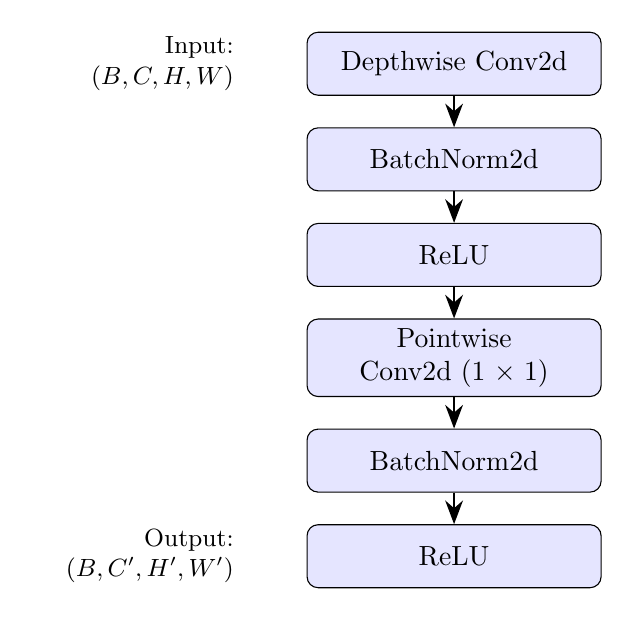
\begin{tikzpicture}[
    block/.style={rectangle, draw, fill=blue!10, text width=3.5cm,
                  text centered, rounded corners, minimum height=0.8cm},
    arrow/.style={-{Stealth[length=3mm]}, thick}
]
    \node[block] (dw) {Depthwise Conv2d};
    \node[block, below=0.4cm of dw] (bn1) {BatchNorm2d};
    \node[block, below=0.4cm of bn1] (relu1) {ReLU};
    \node[block, below=0.4cm of relu1] (pw) {Pointwise Conv2d ($1\times1$)};
    \node[block, below=0.4cm of pw] (bn2) {BatchNorm2d};
    \node[block, below=0.4cm of bn2] (relu2) {ReLU};

    \draw[arrow] (dw) -- (bn1);
    \draw[arrow] (bn1) -- (relu1);
    \draw[arrow] (relu1) -- (pw);
    \draw[arrow] (pw) -- (bn2);
    \draw[arrow] (bn2) -- (relu2);

    \node[left=0.8cm of dw, text width=2.5cm, font=\small, align=right]
        {Input: $(B, C, H, W)$};
    \node[left=0.8cm of relu2, text width=2.5cm, font=\small, align=right]
        {Output: $(B, C', H', W')$};
\end{tikzpicture}
\end{center}

\subsection{Full DSCNN-L Architecture}

The complete DSCNN-L model (276 channels, following Rusci et al.\ \texttt{model\_size\_info\_DSCNNL})
consists of 1 initial convolution + 5 depthwise separable blocks:

\begin{itemize}
    \item \textbf{Initial Conv:} Conv2d$(1, 276, \text{kernel}=(10,4), \text{stride}=(2,1))$ + BN + ReLU
    \item \textbf{DS Block 1:} stride $(2,2)$; \textbf{DS Blocks 2--5:} stride $(1,1)$
    \item \textbf{DS Block 5 (last):} DW still uses BN+ReLU; only post-PW uses LayerNorm(\texttt{elementwise\_affine=False})
    \item \textbf{Average Pooling} $\rightarrow$ Flatten $\rightarrow$ output $(B, 276)$
    \item \textbf{No Linear projection:} embedding\_dim = channel count = 276
    \item \textbf{L2 Normalization:} applied \emph{externally} in the training wrapper (\texttt{ReprModel})
\end{itemize}

\begin{equation}
    \hat{e} = \frac{e}{\|e\|_2}
    \label{eq:l2norm}
\end{equation}

The L2 normalization in \cref{eq:l2norm} is crucial: it ensures all
embeddings lie on the unit hypersphere, making L2 distance equivalent to
cosine distance up to a constant factor.

Three feature extraction modes are available: \texttt{CONV} (raw convolution
output), \texttt{RELU} (after activation), and \texttt{NORM} (after L2
normalization). \texttt{NORM} achieves the best performance \cite{rusci2023}.


\section{Prototypical Networks}
\label{sec:protonet}

Prototypical Networks \cite{snell2017prototypical} learn an embedding space
where classification is performed by computing distances to class prototypes.

\subsection{Core Idea}

Let $f_\theta : \mathbb{R}^D \rightarrow \mathbb{R}^M$ be a neural network
(our DSCNN encoder) that maps input samples to an $M$-dimensional embedding
space. For each class $k$ with support set
$S_k = \{(x_i, y_i)\}_{i=1}^{|S_k|}$ where $y_i = k$, the
\textbf{prototype} $c_k$ is the mean of embedded support samples:

\begin{equation}
    c_k = \frac{1}{|S_k|} \sum_{(x_i, y_i) \in S_k} f_\theta(x_i)
    \label{eq:prototype}
\end{equation}

Given a query sample $x_q$, classification is based on the nearest prototype:
\begin{equation}
    p_\theta(y = k \mid x_q) =
    \frac{\exp(-d(f_\theta(x_q), c_k))}
         {\sum_{k'} \exp(-d(f_\theta(x_q), c_{k'}))}
    \label{eq:proto_softmax}
\end{equation}
where $d(\cdot, \cdot)$ is the squared Euclidean (L2) distance.

\subsection{Episodic Training}

Training mimics the few-shot scenario through \textbf{episodic batching}.
Each episode constructs an $N$-way $K$-shot task:

\begin{enumerate}
    \item Sample $N$ classes from training set
    \item For each class, sample $K$ support examples and $Q$ query examples
    \item Compute prototypes from support set (\cref{eq:prototype})
    \item Classify queries and compute loss
\end{enumerate}

The support and query sets for episode $e$ are:
\begin{align}
    S_e &= \bigcup_{c \in C_e} \{(x_i^c, c)\}_{i=1}^{K} \\
    Q_e &= \bigcup_{c \in C_e} \{(x_j^c, c)\}_{j=K+1}^{K+Q}
\end{align}

\section{Triplet Loss}
\label{sec:triplet}

Instead of the standard prototypical loss, our system uses \textbf{Triplet
Loss} \cite{rusci2023} which directly optimizes the embedding space geometry:

\begin{equation}
    \mathcal{L}_{TL} = \frac{1}{N_t} \sum_{i=1}^{N_t}
    \max\left(0, \; d(x_i, x_i^+) - d(x_i, x_i^-) + m\right)
    \label{eq:triplet}
\end{equation}

where:
\begin{itemize}
    \item $x_i$ is the \textbf{anchor} sample
    \item $x_i^+$ is a \textbf{positive} sample (same class as anchor)
    \item $x_i^-$ is a \textbf{negative} sample (different class)
    \item $m = 0.5$ is the \textbf{margin}
    \item $d(\cdot, \cdot)$ is the L2 distance
\end{itemize}

\textbf{Intuition:} The loss pushes the anchor closer to positive samples
and farther from negative samples by at least margin $m$. When the constraint
is already satisfied, the loss is zero (hinge loss behavior).

\begin{center}
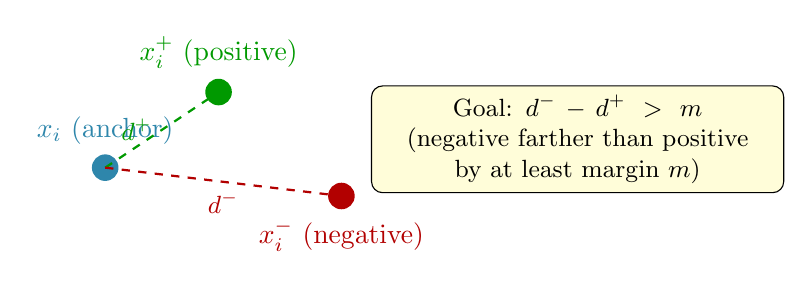
\begin{tikzpicture}[scale=1.2]
    % Anchor
    \fill[corecolor] (0, 0) circle (4pt) node[above=5pt] {$x_i$ (anchor)};
    % Positive
    \fill[green!60!black] (1.2, 0.8) circle (4pt)
        node[above=5pt] {$x_i^+$ (positive)};
    % Negative
    \fill[red!70!black] (2.5, -0.3) circle (4pt)
        node[below=5pt] {$x_i^-$ (negative)};

    % Distance lines
    \draw[thick, green!60!black, dashed] (0,0) -- (1.2, 0.8)
        node[midway, left, font=\small] {$d^+$};
    \draw[thick, red!70!black, dashed] (0,0) -- (2.5, -0.3)
        node[midway, below, font=\small] {$d^-$};

    % Constraint annotation
    \node[draw, rounded corners, fill=yellow!15, text width=5cm,
          font=\small, align=center] at (5, 0.3)
        {Goal: $d^- - d^+ > m$ \\ (negative farther than positive \\ by at
         least margin $m$)};
\end{tikzpicture}
\end{center}

\subsection{Training Configuration}

\begin{table}[h]
\centering
\caption{Training hyperparameters}
\label{tab:training_config}
\begin{tabular}{ll}
\toprule
\textbf{Parameter} & \textbf{Value} \\
\midrule
Loss function & Triplet Loss \\
Margin $m$ & 0.5 \\
Batch composition & 20 samples $\times$ 80 classes \\
Optimizer & Adam \\
Learning rate & 0.001 (StepLR, step\_size=20, $\gamma_{\text{decay}}=0.5$) \\
Epochs & 40 \\
Episodes per epoch & 400 \\
Training dataset & MSWC English (top 450 words; 50 held for validation) \\
Noise augmentation & DEMAND, $p=0.95$, fixed SNR${}=5$\,dB \\
\bottomrule
\end{tabular}
\end{table}


\section{Open-Set Classification}
\label{sec:openset}

Open-set classification extends standard classification by adding the ability
to \textbf{reject unknown inputs}---samples that do not belong to any enrolled
keyword class.

\subsection{Open Nearest Class Mean (openNCM)}

The openNCM classifier \cite{rusci2023} estimates an unknown class prototype
$c_0$ using $K$ random samples from the target domain that do not belong to
user-defined classes. Classification uses softmax over $(N+1)$ distances.

\subsection{Direct L2 Distance Classification (Our Approach)}

Our approach eliminates the probability normalization step and uses L2
distances directly:

\begin{equation}
    d_k = \|f_\theta(x_q) - c_k\|_2, \quad k = 1, \ldots, N
    \label{eq:l2dist}
\end{equation}

\begin{equation}
    \hat{y} = \begin{cases}
        \displaystyle\arg\min_k d_k & \text{if } \min_k d_k \leq \gamma \\
        \text{unknown} & \text{otherwise}
    \end{cases}
    \label{eq:direct_classify}
\end{equation}

where $\gamma$ is the acceptance threshold (radius).

\begin{center}
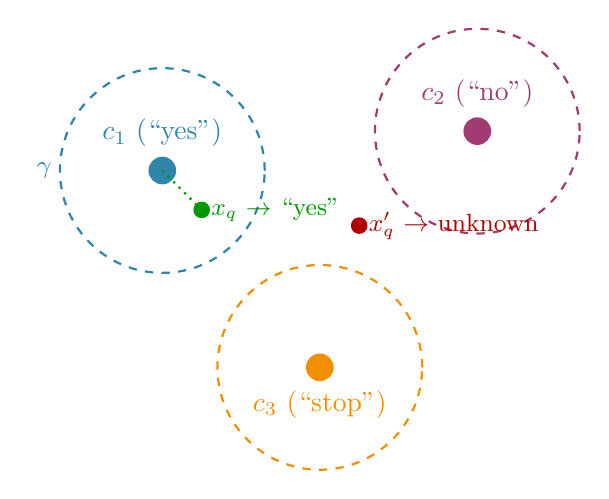
\begin{tikzpicture}[scale=1.0]
    % Prototypes
    \fill[corecolor] (-2, 1) circle (5pt) node[above=5pt] {$c_1$ (``yes'')};
    \fill[ext1color] (2, 1.5) circle (5pt) node[above=5pt] {$c_2$ (``no'')};
    \fill[ext2color] (0, -1.5) circle (5pt) node[below=5pt] {$c_3$ (``stop'')};

    % Acceptance radii
    \draw[corecolor, thick, dashed] (-2, 1) circle (1.3cm);
    \draw[ext1color, thick, dashed] (2, 1.5) circle (1.3cm);
    \draw[ext2color, thick, dashed] (0, -1.5) circle (1.3cm);

    % Threshold label
    \node[font=\small, corecolor] at (-3.5, 1) {$\gamma$};

    % Query - accepted
    \fill[green!60!black] (-1.5, 0.5) circle (3pt)
        node[right, font=\small] {$x_q$ $\rightarrow$ ``yes''};

    % Query - rejected
    \fill[red!70!black] (0.5, 0.3) circle (3pt)
        node[right, font=\small] {$x_q'$ $\rightarrow$ unknown};

    % Distance line
    \draw[green!60!black, dotted, thick] (-2,1) -- (-1.5, 0.5);
\end{tikzpicture}
\end{center}

\textbf{Advantages over probability-based approach:}
\begin{itemize}
    \item Threshold $\gamma$ has geometric meaning (acceptance radius)
    \item No dependency on virtual ``unknown'' prototype computation
    \item Better performance: AUC 0.95 vs 0.94, ACC@5\%FAR 0.81 vs 0.76
          (reference results from \cite{binh2025})
\end{itemize}


\section{Voice Activity Detection (VAD)}

VAD determines whether a given audio segment contains human speech. Our
system uses \textbf{Silero VAD}, a lightweight pre-trained model that
processes 32ms audio chunks (512 samples at 16kHz) and outputs a speech
probability $p \in [0, 1]$.

Speech is detected when $p > \tau_{vad}$ (default $\tau_{vad} = 0.5$).

\section{Speaker Verification with ECAPA-TDNN}

ECAPA-TDNN (Emphasized Channel Attention, Propagation and Aggregation in
TDNN) is a state-of-the-art speaker embedding model that produces 192-dimensional
speaker representations \cite{speechbrain}. Speaker verification compares
cosine similarity between enrolled and query speaker embeddings:

\begin{equation}
    \text{similarity}(e_{enrolled}, e_{query}) =
    \frac{e_{enrolled} \cdot e_{query}}
         {\|e_{enrolled}\|_2 \cdot \|e_{query}\|_2}
    \label{eq:cosine_sim}
\end{equation}

The query is accepted if $\text{similarity} > \tau_{spk}$ (threshold).


% ============================================================
% CHAPTER 3: PROPOSED SYSTEM
% ============================================================
\chapter{Proposed System Design}

\section{System Overview}

Our system follows a modular pipeline architecture with clearly separated
concerns: a \textbf{core KWS engine} (mandatory), two \textbf{extensions}
(noise robustness and streaming), and one \textbf{optional module} (speaker
verification).

\begin{figure}[h]
\centering
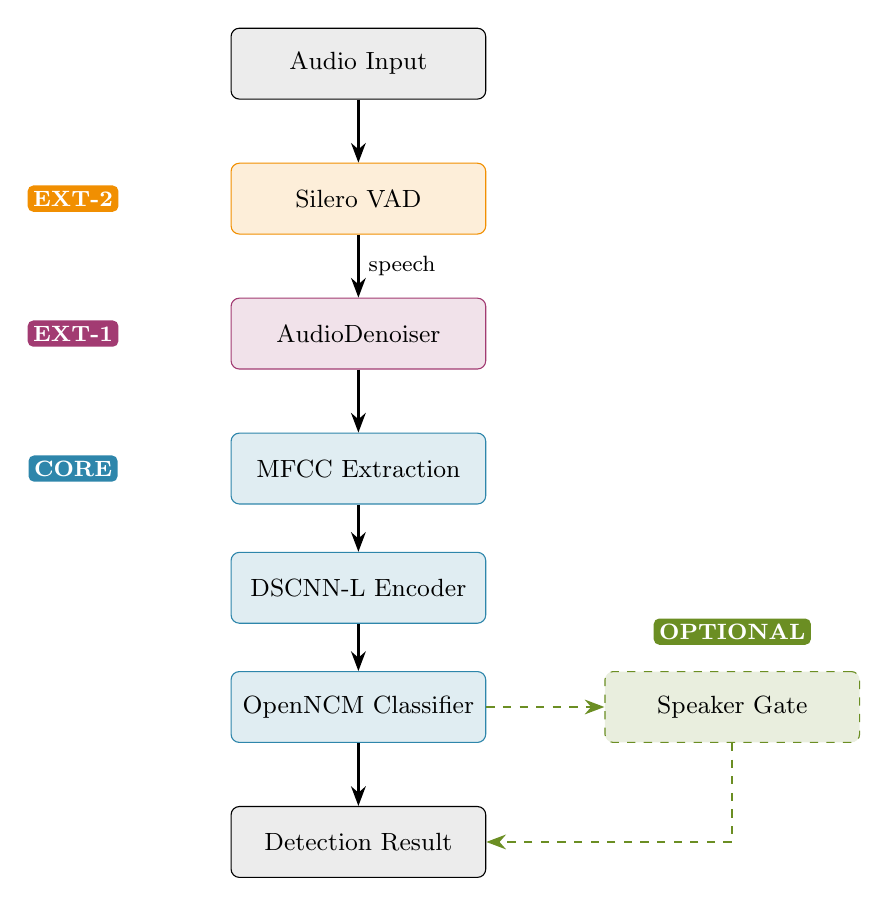
\begin{tikzpicture}[
    node distance=0.6cm and 0.8cm,
    block/.style={rectangle, draw, rounded corners=3pt, minimum height=0.9cm,
                  text width=3cm, text centered, font=\small},
    core/.style={block, fill=corecolor!15, draw=corecolor},
    ext1/.style={block, fill=ext1color!15, draw=ext1color},
    ext2/.style={block, fill=ext2color!15, draw=ext2color},
    opt/.style={block, fill=optcolor!15, draw=optcolor, dashed},
    arrow/.style={-{Stealth[length=2.5mm]}, thick},
    optarrow/.style={-{Stealth[length=2.5mm]}, thick, dashed, optcolor},
    label/.style={font=\footnotesize\bfseries, text=white, rounded corners=2pt,
                  inner sep=2pt}
]
    % Input
    \node[block, fill=gray!15] (input) {Audio Input};

    % Extension 2: Streaming
    \node[ext2, below=0.8cm of input] (vad) {Silero VAD};

    % Extension 1: Denoising
    \node[ext1, below=0.8cm of vad] (denoise) {AudioDenoiser};

    % Core pipeline
    \node[core, below=0.8cm of denoise] (mfcc) {MFCC Extraction};
    \node[core, below=0.6cm of mfcc] (encoder) {DSCNN-L Encoder};
    \node[core, below=0.6cm of encoder] (classify) {OpenNCM Classifier};

    % Optional
    \node[opt, right=1.5cm of classify] (speaker) {Speaker Gate};

    % Output
    \node[block, fill=gray!15, below=0.8cm of classify] (result) {Detection Result};

    % Arrows
    \draw[arrow] (input) -- (vad);
    \draw[arrow] (vad) -- node[right, font=\footnotesize] {speech} (denoise);
    \draw[arrow] (denoise) -- (mfcc);
    \draw[arrow] (mfcc) -- (encoder);
    \draw[arrow] (encoder) -- (classify);
    \draw[arrow] (classify) -- (result);
    \draw[optarrow] (classify.east) -- (speaker.west);
    \draw[optarrow] (speaker.south) |- (result.east);

    % Labels
    \node[label, fill=corecolor] at ([xshift=-2cm]mfcc.west) {CORE};
    \node[label, fill=ext1color] at ([xshift=-2cm]denoise.west) {EXT-1};
    \node[label, fill=ext2color] at ([xshift=-2cm]vad.west) {EXT-2};
    \node[label, fill=optcolor] at ([yshift=0.5cm]speaker.north) {OPTIONAL};

\end{tikzpicture}
\caption{System architecture. Solid lines are mandatory pipeline components.
         Dashed lines indicate the optional speaker verification gate.}
\label{fig:architecture}
\end{figure}


\section{Three-Phase Workflow}

The system operates in three phases:

\subsection{Phase A: Training (Offline, One-time)}

The DSCNN encoder $f_\theta$ is trained on the MSWC English dataset using
episodic Triplet Loss (\cref{sec:triplet}). After training, the encoder
weights are \textbf{frozen}---they are never modified again.

\subsection{Phase B: Enrollment (Per-user, Few-shot)}

Users provide $K$ audio samples (typically $K = 3$--$5$) for each desired
keyword. These are processed through the frozen encoder to compute prototypes:

\begin{equation}
    c_k = \frac{1}{K} \sum_{i=1}^{K} f_\theta(x_i^{(k)})
\end{equation}

\subsection{Phase C: Inference}

For each incoming query, the system computes L2 distances to all prototypes
and applies the open-set decision rule (\cref{eq:direct_classify}).


\section{Core KWS Pipeline}

\begin{algorithm}[h]
\caption{Few-Shot Open-Set KWS Inference}
\label{alg:kws_inference}
\begin{algorithmic}[1]
\Require Audio sample $x_q$, prototypes $\{c_k\}_{k=1}^N$, threshold $\gamma$
\Ensure Predicted keyword or ``unknown''
\State $\text{mfcc} \gets \text{MFCCExtract}(x_q)$
    \Comment{10 features, shape $(B, 1, 47, 10)$}
\State $e_q \gets f_\theta(\text{mfcc})$
    \Comment{DSCNN embedding, L2-normalized}
\For{$k = 1$ to $N$}
    \State $d_k \gets \|e_q - c_k\|_2$
\EndFor
\State $k^* \gets \arg\min_k d_k$
\If{$d_{k^*} \leq \gamma$}
    \State \Return keyword $k^*$ with distance $d_{k^*}$
\Else
    \State \Return ``unknown''
\EndIf
\end{algorithmic}
\end{algorithm}

\section{Extension 1: Noise Robustness}

Noise robustness is achieved through two complementary strategies:

\subsection{Training-time: Noise Augmentation}

During training, clean audio is mixed with background noise from the DEMAND
dataset:
\begin{equation}
    x_{noisy} = x_{clean} + \alpha \cdot x_{noise}, \quad
    \alpha = \frac{\text{RMS}(x_{clean})}{\text{RMS}(x_{noise}) \cdot 10^{\text{SNR}/20}}
\end{equation}
where SNR is fixed at 5\,dB (following Rusci et al.\ \texttt{noise\_snr=5}) with probability $p = 0.95$.
Note: RMS normalization is required because clean and noise signals have different power levels.

\subsection{Inference-time: Audio Denoising}

Before MFCC extraction, an optional denoising step removes background noise:

\begin{itemize}
    \item \textbf{Spectral Gating} (fast, CPU): Statistical noise reduction
          using the \texttt{noisereduce} library
    \item \textbf{SepformerSeparation} (accurate, GPU): Neural speech
          enhancement using SpeechBrain pre-trained models
\end{itemize}

\textbf{Benchmark plan:} Evaluate KWS accuracy at SNR levels 0, 5, 10, 20 dB
and clean conditions, before and after denoising.


\section{Extension 2: Streaming Inference}

\subsection{Sliding Window Detection}

For streaming scenarios, continuous audio is processed using overlapping
windows:

\begin{itemize}
    \item \textbf{Window size:} 16,000 samples (1 second at 16kHz)
    \item \textbf{Stride:} 8,000 samples (0.5 second, 50\% overlap)
    \item \textbf{Buffer:} Ring buffer (\texttt{collections.deque})
\end{itemize}

\subsection{VAD Integration}

Silero VAD pre-filters audio chunks (512 samples = 32ms each). KWS inference
is only triggered when speech is detected, saving computational resources.

\begin{algorithm}[h]
\caption{Streaming KWS with VAD}
\label{alg:streaming}
\begin{algorithmic}[1]
\Require Audio stream, VAD model, KWS model, window size $W$, stride $S$
\State $\text{buffer} \gets \text{empty deque}$
\While{audio stream is active}
    \State $\text{chunk} \gets \text{read\_audio}(512)$
        \Comment{32ms chunk}
    \If{$\text{VAD}(\text{chunk}) = \text{True}$}
        \State $\text{buffer.append(chunk)}$
        \If{$|\text{buffer}| \geq W$}
            \State $\text{window} \gets \text{buffer}[0:W]$
            \State $\text{result} \gets \text{KWS\_Inference}(\text{window})$
                \Comment{Alg. \ref{alg:kws_inference}}
            \State $\text{buffer} \gets \text{buffer}[S:]$
                \Comment{slide by stride}
            \If{result $\neq$ ``unknown''}
                \State \textbf{emit} detection event
            \EndIf
        \EndIf
    \EndIf
\EndWhile
\end{algorithmic}
\end{algorithm}

\subsection{Latency Budget}

\begin{table}[h]
\centering
\caption{Target latency for each pipeline component}
\label{tab:latency}
\begin{tabular}{lr}
\toprule
\textbf{Component} & \textbf{Target Latency} \\
\midrule
VAD per chunk (32ms audio) & $< 5$ ms \\
Denoising (1 sec audio) & $< 30$ ms \\
MFCC extraction & $< 5$ ms \\
DSCNN inference & $< 10$ ms \\
Classifier decision & $< 1$ ms \\
Speaker verification & $< 20$ ms \\
\midrule
\textbf{Total end-to-end} & $\mathbf{< 71}$ \textbf{ms} \\
\bottomrule
\end{tabular}
\end{table}


\section{Optional: Speaker Verification Gate}

After KWS detects a keyword, an optional speaker gate verifies the speaker
identity:

\begin{equation}
    \hat{y}_{final} = \begin{cases}
        \hat{y}_{kws} & \text{if } \text{sim}(e_{owner}, e_{query}) > \tau_{spk} \\
        \text{rejected} & \text{otherwise}
    \end{cases}
\end{equation}

This is strictly \textbf{optional}---the system functions normally without it.
It adds personalization (``only respond to the device owner'').


% ============================================================
% CHAPTER 4: EVALUATION PLAN
% ============================================================
\chapter{Evaluation Plan}

\section{Datasets}

\subsection{Google Speech Commands v2 (GSC)}

\begin{itemize}
    \item 105,829 utterances of 35 English words by 2,618 speakers
    \item 1-second WAV files at 16kHz sampling rate
    \item Used for \textbf{testing} (enrollment + evaluation)
    \item Pre-split into train/dev/test via filename hash (8:1:1)
\end{itemize}

\textbf{Word partitions (Fixed protocol):}
\begin{itemize}
    \item \textbf{GSC+ (10 positive):} yes, no, up, down, left, right, on,
          off, stop, go
    \item \textbf{GSC$-$ (20 negative):} remaining words (unknown class)
    \item \textbf{Excluded (5):} backward, forward, visual, follow, learn
          (reserved for openNCM unknown prototype)
\end{itemize}

\subsection{Multilingual Spoken Words Corpus (MSWC)}

\begin{itemize}
    \item $\sim$22.5 million utterances across 50 languages
    \item Used for \textbf{training} the DSCNN encoder
    \item English subset: top 500 words by utterance count (450 for training, 50 for validation)
    \item Evaluation subset: 263 words (min 1000 utterances each, excluding
          training words)
\end{itemize}

\subsection{DEMAND Noise Dataset}

Background noise recordings for data augmentation during training.

\section{Evaluation Metrics}

\subsection{Detection Error Tradeoff (DET) Curves}

Per-class DET curves plot False Acceptance Rate (FAR) against False Rejection
Rate (FRR) across different thresholds. The \textbf{mean DET curve} averages
across all keyword classes:

\begin{align}
    \text{FAR} &= \frac{\text{FP}}{\text{FP} + \text{TN}} \\
    \text{FRR} &= 1 - \text{TPR} = \frac{\text{FN}}{\text{TP} + \text{FN}}
\end{align}

\subsection{Area Under ROC Curve (AUC)}

Measures overall binary discrimination ability (keyword vs. non-keyword).

\subsection{ACC@5\%FAR}

Classification accuracy within target keywords at the operating point where
FAR = 5\%.

\section{Evaluation Protocols}

\begin{table}[h]
\centering
\caption{Evaluation protocols by priority}
\label{tab:protocols}
\begin{tabular}{llll}
\toprule
\textbf{Priority} & \textbf{Protocol} & \textbf{Positive} & \textbf{Negative} \\
\midrule
Mandatory & GSC Fixed & 10 fixed words & 20 fixed words \\
Mandatory & GSC Randomized & 10 random/run & 20 random/run \\
Extended & MSWC Randomized & 5 random & 50 random \\
\bottomrule
\end{tabular}
\end{table}

\textbf{Mandatory:} Average over 5 runs. Report mean DET, AUC, ACC@5\%FAR. \\
\textbf{Extended:} Average over 10 runs. Add FRR@5\%FAR.

\section{No Data Leakage Guarantee}

\begin{itemize}
    \item Encoder trained on MSWC English (top 450 words; 50 held for validation)
    \item Evaluation performed on GSC (35 entirely different words)
    \item Enrollment, calibration/validation, and test use separate splits
    \item Test queries are never used to create prototypes or select thresholds
\end{itemize}


% ============================================================
% CHAPTER 5: IMPLEMENTATION PLAN
% ============================================================
\chapter{Implementation Plan}

\section{Technology Stack}

\begin{table}[h]
\centering
\caption{Technology stack}
\label{tab:techstack}
\begin{tabular}{ll}
\toprule
\textbf{Component} & \textbf{Technology} \\
\midrule
Framework & PyTorch 2.0+ \\
Audio I/O & torchaudio (primary), librosa (fallback) \\
Feature extraction & torchaudio.transforms.MFCC \\
VAD & Silero VAD v6 \\
Denoising & noisereduce (CPU), SpeechBrain (GPU) \\
Speaker verification & SpeechBrain ECAPA-TDNN \\
Web demo & Gradio \\
Configuration & PyYAML \\
Experiment tracking & TensorBoard \\
\bottomrule
\end{tabular}
\end{table}

\section{Timeline}

\begin{table}[h]
\centering
\caption{Implementation timeline with milestones and priorities}
\label{tab:timeline}
\begin{tabular}{clll}
\toprule
\textbf{Week} & \textbf{Phase} & \textbf{Deliverable} & \textbf{Priority} \\
\midrule
1 & Setup + Pipeline & MFCC $\to$ DSCNN $\to$ embedding &
    \textcolor{corecolor}{\textbf{CORE}} \\
2 & Training + Classifier & Trained model + enroll/predict &
    \textcolor{corecolor}{\textbf{CORE}} \\
3 & Evaluation & Results table + DET curves &
    \textcolor{corecolor}{\textbf{CORE}} \\
\midrule
\multicolumn{4}{c}{\textit{--- Safe Stop Point: complete thesis achievable ---}} \\
\midrule
4 & Denoising & SNR benchmark table &
    \textcolor{ext1color}{\textbf{EXT-1}} \\
5 & Streaming + VAD & Sliding window on long audio &
    \textcolor{ext2color}{\textbf{EXT-2}} \\
6 & Speaker Verify & ``Owner-only'' demo &
    \textcolor{optcolor}{\textbf{OPTIONAL}} \\
7 & Gradio Demo & 3-tab web application &
    DEMO \\
8 & Documentation & Thesis report + defense slides &
    DOCS \\
\bottomrule
\end{tabular}
\end{table}

\section{Risk Management: Cut-Loss Strategy}

If behind schedule, cut in this order (bottom-up):
\begin{enumerate}
    \item \textbf{Cut first:} Speaker verification (optional, does not affect
          core)
    \item \textbf{Cut second:} Real-time microphone streaming (keep offline
          sliding window)
    \item \textbf{Cut third:} Denoising module (keep noise augmentation
          during training)
    \item \textbf{Never cut:} Core KWS + Evaluation + Offline demo
\end{enumerate}


% ============================================================
% CHAPTER 6: EXPECTED RESULTS
% ============================================================
\chapter{Expected Results and Discussion}

\section{Reference Targets}

Based on the reference thesis \cite{binh2025}, we expect results in a similar
range (not necessarily identical due to implementation differences):

\begin{table}[h]
\centering
\caption{Reference performance targets (from \cite{binh2025})}
\label{tab:expected}
\begin{tabular}{lccc}
\toprule
\textbf{Method} & \textbf{AUC} $\uparrow$ &
\textbf{ACC@5\%FAR} $\uparrow$ & \textbf{FRR@5\%FAR} $\downarrow$ \\
\midrule
Probability-based & 0.94 & 0.76 & 0.21 \\
Direct L2 distance & 0.95 & 0.81 & 0.17 \\
\bottomrule
\end{tabular}
\end{table}

\section{Expected Findings}

\begin{enumerate}
    \item Direct L2 distance classification should outperform probability-based
          approaches consistently across operating points.
    \item Randomized word selection protocols will show more realistic (lower)
          performance than fixed partitions.
    \item Denoising will improve accuracy most significantly at low SNR
          (0--5 dB).
    \item Few-shot performance will plateau around 5 enrollment samples per
          keyword.
    \item Streaming inference will show slight accuracy degradation compared
          to offline due to windowing boundary effects.
\end{enumerate}


% ============================================================
% REFERENCES
% ============================================================
\begin{thebibliography}{9}

\bibitem{lopez2021deep}
I.~L{\'o}pez-Espejo, Z.-H.~Tan, J.~Hansen, and J.~Jensen,
``Deep spoken keyword spotting: An overview,''
\textit{IEEE Access}, vol.~10, pp.~4169--4199, 2021.

\bibitem{snell2017prototypical}
J.~Snell, K.~Swersky, and R.~Zemel,
``Prototypical networks for few-shot learning,''
in \textit{Advances in Neural Information Processing Systems}, vol.~30, 2017.

\bibitem{rusci2023}
M.~Rusci and T.~Tuytelaars,
``Few-shot open-set learning for on-device customization of keyword spotting
systems,''
\textit{arXiv preprint arXiv:2306.02161}, 2023.

\bibitem{zhang2017hello}
Y.~Zhang, N.~Suda, L.~Lai, and V.~Chandra,
``Hello edge: Keyword spotting on microcontrollers,''
\textit{arXiv preprint arXiv:1711.07128}, 2017.

\bibitem{binh2025}
P.~T.~Binh,
``Enhanced evaluation protocols for few-shot open-set keyword spotting
systems,''
Master's thesis, University of Science and Technology of Hanoi, 2025.

\bibitem{warden2018}
P.~Warden,
``Speech commands: A dataset for limited-vocabulary speech recognition,''
\textit{arXiv preprint arXiv:1804.03209}, 2018.

\bibitem{mazumder2021mswc}
M.~Mazumder \textit{et al.},
``Multilingual spoken words corpus,''
in \textit{NeurIPS Datasets and Benchmarks Track}, 2021.

\bibitem{speechbrain}
SpeechBrain Team,
``SpeechBrain: A general-purpose speech toolkit,''
2021. [Online]. Available: \url{https://speechbrain.github.io}

\end{thebibliography}

\end{document}
